% Placeholder: plain article class so the outline compiles anywhere.
% TODO: switch to the venue template once the venue is decided, e.g. Springer LNCS
% for MICCAI:
%   \documentclass[runningheads]{llncs}
% (and remove geometry / adjust the bibliography style to splncs04).
\documentclass[11pt]{article}

\usepackage[utf8]{inputenc}
\usepackage[T1]{fontenc}
\usepackage[margin=1in]{geometry}
\usepackage{amsmath,amssymb}
\usepackage{booktabs}
\usepackage{graphicx}
\usepackage{xcolor}
\usepackage{hyperref}

\newcommand{\todo}[1]{\textcolor{red}{[TODO: #1]}}
\newcommand{\expid}[1]{\texttt{#1}}
% Result macros generated by scripts/08_aggregate_results.py (never typed by hand).
% GENERATED by scripts/08_aggregate_results.py from results/. Do not edit.

\newcommand{\resRCMOneStudentAllocatedGpuBytesAfterLoad}{7528507904.000}
\newcommand{\resRCMOneStudentGenerateTokensPerSecond}{8.484}
\newcommand{\resRCMOneStudentParameterDropMatches}{1.000}
\newcommand{\resRCMOneStudentParams}{3754622976.000}
\newcommand{\resRCMOneStudentPeakGpuBytesGenerate}{7569169920.000}
\newcommand{\resRCMOneStudentPeakGpuBytesScoring}{7851811328.000}
\newcommand{\resRCMOneStudentPredictedYesFraction}{0.000}
\newcommand{\resRCMOneStudentRemovalExpectedDropBytes}{154153984.000}
\newcommand{\resRCMOneStudentRemovalMeasuredDropBytes}{154153984.000}
\newcommand{\resRCMOneStudentRemovedLayerParameters}{77076992.000}
\newcommand{\resRCMOneStudentScoresChangeAfterRemoval}{1.000}
\newcommand{\resRCMOneStudentScoresFinite}{1.000}
\newcommand{\resRCMOneStudentScoresFiniteAfterRemoval}{1.000}
\newcommand{\resRCMOneStudentScoringSecondsPerProbe}{0.199}
\newcommand{\resRCMOneStudentYesNoProbabilityMass}{0.999}
\newcommand{\resRCMOneTeacherAllocatedGpuBytesAfterLoad}{16601989632.000}
\newcommand{\resRCMOneTeacherGenerateTokensPerSecond}{4.479}
\newcommand{\resRCMOneTeacherParams}{8292166656.000}
\newcommand{\resRCMOneTeacherPeakGpuBytesGenerate}{16694575104.000}
\newcommand{\resRCMOneTeacherPeakGpuBytesScoring}{17181603328.000}
\newcommand{\resRCMOneTeacherPredictedYesFraction}{0.000}
\newcommand{\resRCMOneTeacherScoresFinite}{1.000}
\newcommand{\resRCMOneTeacherScoringSecondsPerProbe}{0.314}
\newcommand{\resRCMOneTeacherYesNoProbabilityMass}{1.000}
\newcommand{\resRCMOneTokenizersIdentical}{1.000}
\newcommand{\resRCQZeroFpOneSixPeakBytes}{7843649024.000}
\newcommand{\resRCQZeroFpOneSixStateBytes}{7509246624.000}
\newcommand{\resRCQZeroKernelMsTorchAtenLinearWFour}{0.672}
\newcommand{\resRCQZeroKernelMsTorchLinearWFour}{0.238}
\newcommand{\resRCQZeroKernelMsTorchLinearWEight}{0.201}
\newcommand{\resRCQZeroKernelMsTritonVTwoLinearWFour}{0.240}
\newcommand{\resRCQZeroKernelMsTritonVTwoLinearWEight}{0.244}
\newcommand{\resRCQZeroKernelOkAWQBitBLASMlxQuantLinearWFour}{0.000}
\newcommand{\resRCQZeroKernelOkAWQBitBLASMlxQuantLinearWEight}{0.000}
\newcommand{\resRCQZeroKernelOkAWQBitBlasKernelWFour}{0.000}
\newcommand{\resRCQZeroKernelOkAWQBitBlasKernelWEight}{0.000}
\newcommand{\resRCQZeroKernelOkAWQMarlinMlxQuantLinearWFour}{0.000}
\newcommand{\resRCQZeroKernelOkAWQMarlinMlxQuantLinearWEight}{0.000}
\newcommand{\resRCQZeroKernelOkAwqBitBLASLinearWFour}{0.000}
\newcommand{\resRCQZeroKernelOkAwqBitBLASLinearWEight}{0.000}
\newcommand{\resRCQZeroKernelOkAwqExllamaVTwoLinearWFour}{0.000}
\newcommand{\resRCQZeroKernelOkAwqExllamaVTwoLinearWEight}{0.000}
\newcommand{\resRCQZeroKernelOkAwqGEMMLinearWFour}{0.000}
\newcommand{\resRCQZeroKernelOkAwqGEMMLinearWEight}{0.000}
\newcommand{\resRCQZeroKernelOkAwqGEMMTritonLinearWFour}{0.000}
\newcommand{\resRCQZeroKernelOkAwqGEMMTritonLinearWEight}{0.000}
\newcommand{\resRCQZeroKernelOkAwqGEMVFastLinearWFour}{0.000}
\newcommand{\resRCQZeroKernelOkAwqGEMVFastLinearWEight}{0.000}
\newcommand{\resRCQZeroKernelOkAwqGEMVLinearWFour}{0.000}
\newcommand{\resRCQZeroKernelOkAwqGEMVLinearWEight}{0.000}
\newcommand{\resRCQZeroKernelOkAwqGemvFastMlxQuantLinearWFour}{0.000}
\newcommand{\resRCQZeroKernelOkAwqGemvFastMlxQuantLinearWEight}{0.000}
\newcommand{\resRCQZeroKernelOkAwqGemvMlxQuantLinearWFour}{0.000}
\newcommand{\resRCQZeroKernelOkAwqGemvMlxQuantLinearWEight}{0.000}
\newcommand{\resRCQZeroKernelOkAwqMacheteLinearWFour}{0.000}
\newcommand{\resRCQZeroKernelOkAwqMacheteLinearWEight}{0.000}
\newcommand{\resRCQZeroKernelOkAwqMarlinLinearWFour}{0.000}
\newcommand{\resRCQZeroKernelOkAwqMarlinLinearWEight}{0.000}
\newcommand{\resRCQZeroKernelOkAwqMlxQuantLinearWFour}{0.000}
\newcommand{\resRCQZeroKernelOkAwqMlxQuantLinearWEight}{0.000}
\newcommand{\resRCQZeroKernelOkAwqSwordfishLinearWFour}{0.000}
\newcommand{\resRCQZeroKernelOkAwqSwordfishLinearWEight}{0.000}
\newcommand{\resRCQZeroKernelOkAwqTorchLinearWFour}{0.000}
\newcommand{\resRCQZeroKernelOkAwqTorchLinearWEight}{0.000}
\newcommand{\resRCQZeroKernelOkBitBLASLinearWFour}{0.000}
\newcommand{\resRCQZeroKernelOkBitBLASLinearWEight}{0.000}
\newcommand{\resRCQZeroKernelOkBitblasBaseQuantLinearWFour}{0.000}
\newcommand{\resRCQZeroKernelOkBitblasBaseQuantLinearWEight}{0.000}
\newcommand{\resRCQZeroKernelOkBitblasLinearWFour}{0.000}
\newcommand{\resRCQZeroKernelOkBitblasLinearWEight}{0.000}
\newcommand{\resRCQZeroKernelOkBitsAndBytesFourbitLinearWFour}{0.000}
\newcommand{\resRCQZeroKernelOkBitsAndBytesFourbitLinearWEight}{0.000}
\newcommand{\resRCQZeroKernelOkBitsAndBytesLinearWFour}{0.000}
\newcommand{\resRCQZeroKernelOkBitsAndBytesLinearWEight}{0.000}
\newcommand{\resRCQZeroKernelOkBitsAndBytesMlxQuantLinearWFour}{0.000}
\newcommand{\resRCQZeroKernelOkBitsAndBytesMlxQuantLinearWEight}{0.000}
\newcommand{\resRCQZeroKernelOkExllamaVTwoLinearWFour}{0.000}
\newcommand{\resRCQZeroKernelOkExllamaVTwoLinearWEight}{0.000}
\newcommand{\resRCQZeroKernelOkFPEightMlxQuantLinearWFour}{0.000}
\newcommand{\resRCQZeroKernelOkFPEightMlxQuantLinearWEight}{0.000}
\newcommand{\resRCQZeroKernelOkGGUFCppKernelWFour}{0.000}
\newcommand{\resRCQZeroKernelOkGGUFCppKernelWEight}{0.000}
\newcommand{\resRCQZeroKernelOkGGUFCudaKernelWFour}{0.000}
\newcommand{\resRCQZeroKernelOkGGUFCudaKernelWEight}{0.000}
\newcommand{\resRCQZeroKernelOkGGUFMlxQuantLinearWFour}{0.000}
\newcommand{\resRCQZeroKernelOkGGUFMlxQuantLinearWEight}{0.000}
\newcommand{\resRCQZeroKernelOkGGUFTorchLinearWFour}{0.000}
\newcommand{\resRCQZeroKernelOkGGUFTorchLinearWEight}{0.000}
\newcommand{\resRCQZeroKernelOkGGUFTritonKernelWFour}{0.000}
\newcommand{\resRCQZeroKernelOkGGUFTritonKernelWEight}{0.000}
\newcommand{\resRCQZeroKernelOkGPTQBitBLASMlxQuantLinearWFour}{0.000}
\newcommand{\resRCQZeroKernelOkGPTQBitBLASMlxQuantLinearWEight}{0.000}
\newcommand{\resRCQZeroKernelOkGPTQMarlinMlxQuantLinearWFour}{0.000}
\newcommand{\resRCQZeroKernelOkGPTQMarlinMlxQuantLinearWEight}{0.000}
\newcommand{\resRCQZeroKernelOkLLMAwqLinearWFour}{0.000}
\newcommand{\resRCQZeroKernelOkLLMAwqLinearWEight}{0.000}
\newcommand{\resRCQZeroKernelOkLLMAwqMlxQuantLinearWFour}{0.000}
\newcommand{\resRCQZeroKernelOkLLMAwqMlxQuantLinearWEight}{0.000}
\newcommand{\resRCQZeroKernelOkMacheteLinearWFour}{0.000}
\newcommand{\resRCQZeroKernelOkMacheteLinearWEight}{0.000}
\newcommand{\resRCQZeroKernelOkMarlinLinearWFour}{0.000}
\newcommand{\resRCQZeroKernelOkMarlinLinearWEight}{0.000}
\newcommand{\resRCQZeroKernelOkMlxQuantLinearWFour}{0.000}
\newcommand{\resRCQZeroKernelOkMlxQuantLinearWEight}{0.000}
\newcommand{\resRCQZeroKernelOkParoLinearWFour}{0.000}
\newcommand{\resRCQZeroKernelOkParoLinearWEight}{0.000}
\newcommand{\resRCQZeroKernelOkParoMlxQuantLinearWFour}{0.000}
\newcommand{\resRCQZeroKernelOkParoMlxQuantLinearWEight}{0.000}
\newcommand{\resRCQZeroKernelOkParoQuantTritonLinearWFour}{0.000}
\newcommand{\resRCQZeroKernelOkParoQuantTritonLinearWEight}{0.000}
\newcommand{\resRCQZeroKernelOkQQQLinearWFour}{0.000}
\newcommand{\resRCQZeroKernelOkQQQLinearWEight}{0.000}
\newcommand{\resRCQZeroKernelOkQQQMlxQuantLinearWFour}{0.000}
\newcommand{\resRCQZeroKernelOkQQQMlxQuantLinearWEight}{0.000}
\newcommand{\resRCQZeroKernelOkQQQTorchLinearWFour}{0.000}
\newcommand{\resRCQZeroKernelOkQQQTorchLinearWEight}{0.000}
\newcommand{\resRCQZeroKernelOkSwordfishLinearWFour}{0.000}
\newcommand{\resRCQZeroKernelOkSwordfishLinearWEight}{0.000}
\newcommand{\resRCQZeroKernelOkTorchAtenAwqLinearWFour}{0.000}
\newcommand{\resRCQZeroKernelOkTorchAtenAwqLinearWEight}{0.000}
\newcommand{\resRCQZeroKernelOkTorchAtenLinearWFour}{1.000}
\newcommand{\resRCQZeroKernelOkTorchAtenLinearWEight}{0.000}
\newcommand{\resRCQZeroKernelOkTorchFPEightLinearWFour}{0.000}
\newcommand{\resRCQZeroKernelOkTorchFPEightLinearWEight}{0.000}
\newcommand{\resRCQZeroKernelOkTorchFusedAwqLinearWFour}{0.000}
\newcommand{\resRCQZeroKernelOkTorchFusedAwqLinearWEight}{0.000}
\newcommand{\resRCQZeroKernelOkTorchFusedLinearWFour}{0.000}
\newcommand{\resRCQZeroKernelOkTorchFusedLinearWEight}{0.000}
\newcommand{\resRCQZeroKernelOkTorchIntEightAwqLinearWFour}{0.000}
\newcommand{\resRCQZeroKernelOkTorchIntEightAwqLinearWEight}{0.000}
\newcommand{\resRCQZeroKernelOkTorchIntEightLinearWFour}{0.000}
\newcommand{\resRCQZeroKernelOkTorchIntEightLinearWEight}{0.000}
\newcommand{\resRCQZeroKernelOkTorchLinearWFour}{1.000}
\newcommand{\resRCQZeroKernelOkTorchLinearWEight}{1.000}
\newcommand{\resRCQZeroKernelOkTorchQuantEmbeddingsWFour}{0.000}
\newcommand{\resRCQZeroKernelOkTorchQuantEmbeddingsWEight}{0.000}
\newcommand{\resRCQZeroKernelOkTritonVTwoLinearWFour}{1.000}
\newcommand{\resRCQZeroKernelOkTritonVTwoLinearWEight}{1.000}
\newcommand{\resRCQZeroKernelOkWFourAFPEightLinearWFour}{0.000}
\newcommand{\resRCQZeroKernelOkWFourAFPEightLinearWEight}{0.000}
\newcommand{\resRCQZeroKernelOkWFourANVFPFourLinearWFour}{0.000}
\newcommand{\resRCQZeroKernelOkWFourANVFPFourLinearWEight}{0.000}
\newcommand{\resRCQZeroWFourAgreementWithFpOneSix}{1.000}
\newcommand{\resRCQZeroWFourGptqSeconds}{507.678}
\newcommand{\resRCQZeroWFourKernelsOk}{1.000}
\newcommand{\resRCQZeroWFourPeakBytes}{3797138944.000}
\newcommand{\resRCQZeroWFourStateBytes}{3405009312.000}
\newcommand{\resRCQZeroWEightAgreementWithFpOneSix}{1.000}
\newcommand{\resRCQZeroWEightGptqSeconds}{504.092}
\newcommand{\resRCQZeroWEightKernelsOk}{1.000}
\newcommand{\resRCQZeroWEightPeakBytes}{5197114880.000}
\newcommand{\resRCQZeroWEightStateBytes}{4803105312.000}
\newcommand{\resRCQZeroWEightaEightAgreementWithFpOneSix}{1.000}
\newcommand{\resRCQZeroWEightaEightKernelsOk}{1.000}
\newcommand{\resRCQZeroWEightaEightPeakBytes}{5073484288.000}
\newcommand{\resRCQZeroWEightaEightStateBytes}{4734714528.000}


\title{What Compression Forgets: Pruning vs.\ Quantization vs.\ Distillation in
Medical Vision-Language Models, and a Clinically Weighted Pruning Criterion for
Preserving Small Findings}
% TODO: anonymise for double-blind review.
\author{Amir \and Soheil Jafari \and Farzan \\ \todo{affiliations}}
\date{}

\begin{document}
\maketitle

\begin{abstract}
% TODO: write last. About 150-250 words (check venue limit).
% 1. Problem: compressed medical VLMs are judged by average accuracy, which can hide
%    loss of small-lesion recall, rare-finding recall, image reliance and calibration.
% 2. What we do: compare pruning, quantization and distillation of one medical VLM at
%    the same MEASURED memory/latency budget (E0-E9).
% 3. Method: clinically weighted structured-pruning criterion (E7).
% 4. Findings: TODO (fill from Table~\ref{tab:main}, primary endpoints at B2).
% 5. Release: open evaluation harness.
\todo{abstract}
\end{abstract}

\section{Introduction}
\label{sec:intro}

% TODO: motivation. Compression is needed to deploy medical VLMs on limited hardware.
% Papers report average accuracy; clinically important failures (small lesions, rare
% findings, answering without looking at the image, overconfidence, hallucinated
% findings) can get worse while average accuracy holds.
\todo{motivation: why average accuracy hides compression harm}

% TODO: research questions.
% RQ1: At a matched measured budget, do compression families with similar average
%      accuracy differ in small-finding recall, rare-finding recall, image reliance,
%      calibration and hallucination?
% RQ2: Which compression family (quantization, distillation, generic pruning,
%      layer pruning) damages which property?
% RQ3: Does a clinically weighted pruning criterion preserve small findings and
%      image reliance better than generic criteria at the same budget?
\todo{RQ1--RQ3}

% TODO: contributions.
% C1 Audit: controlled comparison of E1-E9 at matched measured budgets on hidden
%    metrics, not only accuracy.
% C2 Clinical pruning criterion (E7) with pre-registered finding weights.
% C3 Open evaluation harness (stress tests, mask audit, efficiency checks).
\todo{contributions C1--C3}

\begin{figure}[t]
  \centering
  \fbox{\parbox{0.9\linewidth}{\centering\vspace{3em}
    Placeholder: headline accuracy vs.\ small-finding recall for \expid{E2},
    \expid{E3}, \expid{E5}, \expid{E6}, \expid{E7} at \expid{B2}.\vspace{3em}}}
  \caption{Teaser: compression methods with similar average accuracy differ in
  small-finding recall. Fed by \expid{E2}, \expid{E3}, \expid{E5}--\expid{E7} at
  \expid{B2}.}
  \label{fig:teaser}
\end{figure}

\section{Related Work}
\label{sec:related}

% TODO: write after reading every entry in docs/related_work.md. Re-check all
% bibliographic details before submission.

\subsection{Compression of vision-language models}
% TODO: structured pruning, distillation and quantization of (large) VLMs.
\todo{VLM compression} \cite{lin_mopeclip,huang_structural_pruning_vlm,cai_llavakd,chen_grace}

\subsection{Medical vision-language models and their compression}
% TODO: medical VLMs; compression in medical contexts.
\todo{medical VLMs and their compression} \cite{khan_compression_medical_mllm,qian_medopd,medtokenbudget}

\subsection{What compression forgets}
% TODO: pruning / quantization effects beyond average accuracy (long tail,
% evidence, explanations); position our audit and criterion.
% Hooker et al. (arXiv:1911.05248): the cost of compression falls on a small subset of
% examples, which top-line accuracy hides. Our pre-registered secondary flip analysis
% (2026-10-31) follows it: for each method and budget, the test probes whose answer flips
% between E0 and the compressed model, by finding and by lesion-size stratum (are small
% polyps over-represented among the flips?), with image-bootstrap intervals.
Compression can keep the average accuracy of a model while its errors move to a small set of
examples~\cite{hooker_compressed_forget}; we ask whether, in endoscopy, those examples are the
small lesions (Section~\ref{sec:setup}).
\todo{what compression forgets} \cite{holste_pruning_longtail,khalid_pruning_longtail,ghostq,kim_quantization_evidence}

% Datasets are cited in Section~\ref{sec:setup} (e.g.\ \cite{colonx}).

\section{Method}
\label{sec:method}

\subsection{Study design}
% TODO: one teacher (E0), one student (E1, E2); every compression arm starts from E2
% (or E7 for E8, E0 for E9); all arms are compared at the same MEASURED budget
% (peak memory or latency as a fraction of E2), not parameter count.
\todo{study design}

\subsection{Compression arms}
% TODO: describe E3 (PTQ: W8, W4 via GPTQ/AWQ, W8A8), E4 (QAKD, GRACE-style),
% E5 (magnitude, activation, Taylor), E6 (output-similarity layer pruning), E7 (ours),
% E8 (E7 + 4-bit), E9 (teacher 4-bit).

\begin{table}[t]
  \centering
  \caption{Experiment ladder (\expid{E0}--\expid{E9}) and ablations
  (\expid{A1}--\expid{A6}). Source: \texttt{src/medcompress/registry.py}.}
  \label{tab:ladder}
  \begin{tabular}{llll}
    \toprule
    ID & Description & Starts from & Budgets \\
    \midrule
    \expid{E0} & Teacher, full precision & -- & -- \\
    \expid{E1} & Student, answer fine-tuning & -- & -- \\
    \expid{E2} & Student + offline KD & -- & reference \\
    \expid{E3} & PTQ (W8/W4/W8A8) & \expid{E2} & measured \\
    \expid{E4} & QAKD & -- & measured \\
    \expid{E5} & Generic structured pruning + recovery & \expid{E2} & B1--B3 \\
    \expid{E6} & Output-similarity layer pruning + recovery & \expid{E2} & B1--B3 \\
    \expid{E7} & Clinical pruning (ours) + recovery & \expid{E2} & B1--B3 \\
    \expid{E8} & \expid{E7} + 4-bit PTQ & \expid{E7} & B1--B3 \\
    \expid{E9} & Teacher 4-bit (suppl.) & \expid{E0} & measured \\
    \expid{A1}--\expid{A6} & Criterion ablations & \expid{E2} & B2 \\
    \bottomrule
  \end{tabular}
\end{table}

\subsection{Clinically weighted pruning criterion}
% TODO: units (layers, GQA-consistent head groups, MLP channel groups; projector kept),
% probes, Delta variants, weights, procedure. Keep consistent with
% src/medcompress/compression/pruning/criteria/clinical.py.
For each candidate unit $j$ we compute
\begin{equation}
  I_j = \sum_{c \in C} w_c \, \frac{1}{|X_{\mathrm{cal}}|} \sum_{x \in X_{\mathrm{cal}}} \Delta_j(c, x),
  \label{eq:importance}
\end{equation}
where $\Delta_j(c, x) = \log p_\theta(y_{c,x} \mid x, q_c) - \log p_{\theta \setminus j}(y_{c,x} \mid x, q_c)$
is the drop in log-probability of the correct yes/no answer to the probe $q_c$ when
unit $j$ is ablated, and $w_c = \min(1/\pi_c, \kappa)\, \tau(c)$ combines capped
inverse prevalence and a pre-registered clinical importance tier.
\todo{full definitions, KL variant, procedure}

\begin{figure}[t]
  \centering
  \fbox{\parbox{0.9\linewidth}{\centering\vspace{3em}
    Placeholder: probe $\rightarrow$ ablate $\rightarrow$ score $\rightarrow$ rank
    $\rightarrow$ remove to budget $\rightarrow$ recover $\rightarrow$ mask audit.\vspace{3em}}}
  \caption{Overview of the clinical pruning criterion (\expid{E7}).}
  \label{fig:method}
\end{figure}

\subsection{Shared recovery}
% TODO: identical LoRA + offline KD recovery for all pruning arms (E5, E6, E7,
% A1-A6): same data subset, steps and hyper-parameters; recovery config fingerprint.
\todo{recovery}

\subsection{Mask audit}
% TODO: lesion masked vs area-matched random region masked; lesion-mask effect.
\todo{mask audit}

\section{Experimental Setup}
\label{sec:setup}

\subsection{Models}
% TODO: teacher Qwen2.5-VL-7B-Instruct + Kvasir-VQA-x1 LoRA (D01); student chosen by
% the staged selection over ten Qwen-family models (D05, appendix); fp16 on T4.
\todo{models}

\subsection{Data}
% TODO: Kvasir-VQA-x1 (main QA; validation and test = halves of its official test
% split by image), Kvasir-SEG masks matched by fingerprint, EndoBench external test
% (deduplicated), finding list and prevalence groups (D02).
\todo{data}

\begin{table}[t]
  \centering
  \caption{Data statistics (aggregate counts from the data-preparation run; generated).}
  \label{tab:data}
  % GENERATED by scripts/08_aggregate_results.py from results/. Do not edit.

\begin{tabular}{ll}
\toprule
Quantity & Value \\
\midrule
-- & -- \\
\bottomrule
\end{tabular}

\end{table}

\subsection{Budgets}
% TODO: measurement protocol, hardware, B1-B3 as fractions of E2 peak memory.
\todo{budgets}

\begin{table}[t]
  \centering
  \caption{Measured budgets: \expid{E2} reference and targets \expid{B1}--\expid{B3}.}
  \label{tab:budgets}
  \begin{tabular}{lll}
    \toprule
    Budget & Target fraction of \expid{E2} & Measured peak memory / latency \\
    \midrule
    reference (\expid{E2}) & 1.00 & -- \\
    \expid{B1} & -- & -- \\
    \expid{B2} & -- & -- \\
    \expid{B3} & -- & -- \\
    \bottomrule
  \end{tabular}
\end{table}

\subsection{Metrics}
% TODO: clinical, small findings (lesion-area quartiles), rare findings (prevalence
% groups), image reliance (blank, lesion vs random mask, other patient),
% calibration (ECE, Brier, risk-coverage), hallucination/omission/negation,
% efficiency.
\todo{metrics}

\subsection{Statistics}
% TODO: paired bootstrap 95% CIs, McNemar per finding, Holm correction, mean and SD
% over 3 seeds; primary endpoints pre-registered.
\todo{statistics}

\subsection{Hardware}
% TODO: Kaggle 2x T4 for development, rented GPU (type TODO) for final timing.
\todo{hardware}

\section{Results}
\label{sec:results}

% All numbers come from scripts/08_aggregate_results.py outputs: tables in
% paper/tables/*.tex, figures in paper/figures/*.pdf, and number macros in
% paper/tables/numbers.tex (e.g. \resESevenBTwoSmallFindingRecall).
% Never type a result number in this file; tests/test_paper.py checks it.

\subsection{Headline vs.\ hidden metrics}
% TODO: average accuracy holds while hidden metrics drop (H1).
\todo{headline vs hidden}

\begin{figure}[t]
  \centering
  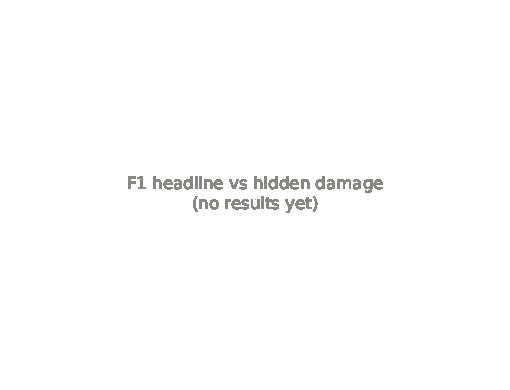
\includegraphics[width=0.48\linewidth]{figures/headline_vs_hidden.pdf}
  \caption{Headline vs.\ hidden damage: drop in accuracy against drop in
  small-finding recall relative to \expid{E2}; points above the diagonal lose
  more on small findings than on accuracy (H1).}
  \label{fig:headline}
\end{figure}

\begin{table}[t]
  \centering
  \caption{Main results: \expid{E2} reference, \expid{E3} (measured footprint) and
  \expid{E5}--\expid{E8} at \expid{B1}--\expid{B3}; mean $\pm$ SD over 3 seeds.}
  \label{tab:main}
  \resizebox{\linewidth}{!}{% GENERATED by scripts/08_aggregate_results.py from results/. Do not edit.

\begin{tabular}{llllll}
\toprule
Budget & Arm & Accuracy & Balanced acc. & Small-finding recall & Lesion-mask effect \\
\midrule
ref & E2 & -- & -- & -- & -- \\
meas. & E3:w8 & -- & -- & -- & -- \\
meas. & E3:w4 & -- & -- & -- & -- \\
meas. & E3:w8a8 & -- & -- & -- & -- \\
B1 & E5:magnitude & -- & -- & -- & -- \\
B1 & E5:activation & -- & -- & -- & -- \\
B1 & E5:taylor & -- & -- & -- & -- \\
B1 & E6 & -- & -- & -- & -- \\
B1 & E7 & -- & -- & -- & -- \\
B1 & E8 & -- & -- & -- & -- \\
B2 & E5:magnitude & -- & -- & -- & -- \\
B2 & E5:activation & -- & -- & -- & -- \\
B2 & E5:taylor & -- & -- & -- & -- \\
B2 & E6 & -- & -- & -- & -- \\
B2 & E7 & -- & -- & -- & -- \\
B2 & E8 & -- & -- & -- & -- \\
B3 & E5:magnitude & -- & -- & -- & -- \\
B3 & E5:activation & -- & -- & -- & -- \\
B3 & E5:taylor & -- & -- & -- & -- \\
B3 & E6 & -- & -- & -- & -- \\
B3 & E7 & -- & -- & -- & -- \\
B3 & E8 & -- & -- & -- & -- \\
\bottomrule
\end{tabular}
}
\end{table}

\subsection{Which compression family damages what}
% TODO: per-metric change relative to E2 (H2).
\todo{family comparison}

\begin{figure}[t]
  \centering
  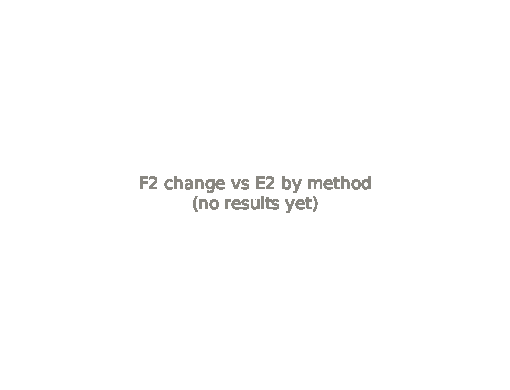
\includegraphics[width=\linewidth]{figures/family_damage.pdf}
  \caption{Change vs.\ \expid{E2} on each metric (rows) for each compressed arm
  (columns).}
  \label{fig:families}
\end{figure}

\begin{figure}[t]
  \centering
  
\includegraphics[width=0.48\linewidth]{figures/budget_curves.pdf}
  \caption{Small-finding recall against measured peak memory (fraction of
  \expid{E2}).}
  \label{fig:budgets}
\end{figure}

\subsection{Clinical vs.\ generic pruning criteria}
% TODO: primary endpoints at B2, E7 vs best of E5 and E6 (H3, Holm-corrected).
\todo{clinical vs generic}

\begin{table}[t]
  \centering
  \caption{Primary comparison at \expid{B2}: \expid{E7} minus the best of
  \expid{E5}/\expid{E6} (chosen on validation); paired bootstrap 95\% CIs and
  Holm-adjusted $p$-values.}
  \label{tab:primary}
  \resizebox{\linewidth}{!}{% GENERATED by scripts/08_aggregate_results.py from results/. Do not edit.

\begin{tabular}{lllll}
\toprule
Comparison & $\Delta$ small-finding recall [95\% CI] & $p_{\mathrm{Holm}}$ & $\Delta$ lesion-mask effect [95\% CI] & $p_{\mathrm{Holm}}$ \\
\midrule
E7 vs best of E5/E6 & -- & -- & -- & -- \\
\bottomrule
\end{tabular}
}
\end{table}

\begin{figure}[t]
  \centering
  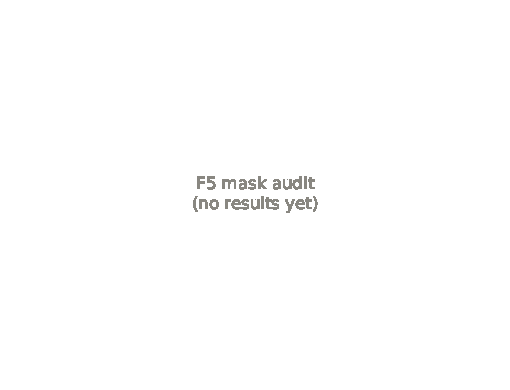
\includegraphics[width=0.48\linewidth]{figures/mask_audit.pdf}
  \caption{Mask audit: answer flip rate when the lesion is masked vs.\ an
  area-matched random region.}
  \label{fig:mask}
\end{figure}

\subsection{Ablations}
% TODO: A1-A6 at B2.
\todo{ablations}

\begin{table}[t]
  \centering
  \caption{Criterion ablations at \expid{B2}.}
  \label{tab:ablations}
  % GENERATED by scripts/08_aggregate_results.py from results/. Do not edit.

\begin{tabular}{lll}
\toprule
Arm & Small-finding recall & Lesion-mask effect \\
\midrule
E7 & -- & -- \\
A1 & -- & -- \\
A2 & -- & -- \\
A3 & -- & -- \\
A4:n32 & -- & -- \\
A4:n64 & -- & -- \\
A4:n128 & -- & -- \\
A4:n256 & -- & -- \\
A5:logprob\_drop & -- & -- \\
A5:kl & -- & -- \\
A6:layers\_only & -- & -- \\
A6:heads\_channels & -- & -- \\
\bottomrule
\end{tabular}

\end{table}

\subsection{Is accuracy a reliable guide?}
% TODO: H4.
\todo{ranking}

\begin{figure}[t]
  \centering
  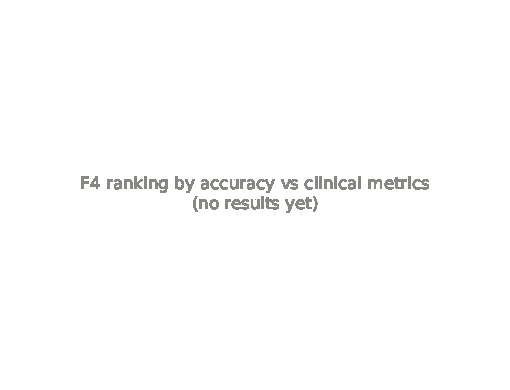
\includegraphics[width=0.48\linewidth]{figures/rank_order.pdf}
  \caption{Rank of each compressed arm by accuracy vs.\ by small-finding recall
  (H4).}
  \label{fig:rank}
\end{figure}

\subsection{Efficiency and external test}
% TODO: measured footprints; low-precision kernel check; external test.
\todo{efficiency}

\begin{table}[t]
  \centering
  \caption{Efficiency on the timing GPU (budget-matched arms at \expid{B2}).}
  \label{tab:efficiency}
  \resizebox{\linewidth}{!}{% GENERATED by scripts/08_aggregate_results.py from results/. Do not edit.

\begin{tabular}{lllllll}
\toprule
Arm & Params & File size & Peak memory & Cold latency (s) & Warm latency (s) & Kernels OK \\
\midrule
E0 & -- & -- & -- & -- & -- & -- \\
E1 & -- & -- & -- & -- & -- & -- \\
E2 & -- & -- & -- & -- & -- & -- \\
E3:w8 & -- & -- & -- & -- & -- & -- \\
E3:w4 & -- & -- & -- & -- & -- & -- \\
E3:w8a8 & -- & -- & -- & -- & -- & -- \\
E4 & -- & -- & -- & -- & -- & -- \\
E5:magnitude & -- & -- & -- & -- & -- & -- \\
E5:activation & -- & -- & -- & -- & -- & -- \\
E5:taylor & -- & -- & -- & -- & -- & -- \\
E6 & -- & -- & -- & -- & -- & -- \\
E7 & -- & -- & -- & -- & -- & -- \\
E8 & -- & -- & -- & -- & -- & -- \\
E9 & -- & -- & -- & -- & -- & -- \\
\bottomrule
\end{tabular}
}
\end{table}

\begin{table}[t]
  \centering
  \caption{External test (deduplicated against training images).}
  \label{tab:external}
  % GENERATED by scripts/08_aggregate_results.py from results/. Do not edit.

\begin{tabular}{llll}
\toprule
Arm & Accuracy & Small-finding recall & Lesion-mask effect \\
\midrule
E0 & -- & -- & -- \\
E2 & -- & -- & -- \\
E3:w8 & -- & -- & -- \\
E3:w4 & -- & -- & -- \\
E3:w8a8 & -- & -- & -- \\
E5:magnitude & -- & -- & -- \\
E5:activation & -- & -- & -- \\
E5:taylor & -- & -- & -- \\
E6 & -- & -- & -- \\
E7 & -- & -- & -- \\
\bottomrule
\end{tabular}

\end{table}

\section{Discussion}
\label{sec:discussion}

\subsection{What to check before deploying a compressed medical model}
% TODO: practical checklist derived from results: small-finding recall, rare-finding
% recall, image reliance tests, calibration, hallucination, measured (not nominal)
% efficiency, low-precision kernel check.
\todo{deployment checklist}

\subsection{Limitations}
% TODO: one model pair and one domain; dataset size and label noise; masks only for
% some findings; budgets on specific hardware; probe-based criterion depends on the
% finding list and weights.
\todo{limitations}

\section{Conclusion}
\label{sec:conclusion}

% TODO: answer RQ1-RQ3 in one paragraph; restate C1-C3; point to the released harness.
\todo{conclusion}


\bibliographystyle{plain}
\bibliography{references}

\appendix
\section{Additional Results and Details}
\label{sec:appendix}

\subsection{Student selection}
\label{app:student-selection}
The student is chosen by successive halving over ten candidate architectures that
share the teacher's tokenizer, so that the cached teacher outputs can be reused
without re-tokenisation. All stages use the validation split only; the test split
is never touched. Stage 0 checks that a candidate fits one 16\,GB GPU and
generates text; stage 1 gives all ten the same short fine-tune; stage 2 retrains
the best five with the full student recipe; stage 3 retrains the best three with
the exact \expid{E2} recipe and two seeds. One candidate is kept. A candidate is
excluded at any stage if it fails one of five gates: it fits the hardware, it uses
the image, it can be compressed (units can be enumerated and removed), its licence
permits the study, and it has seen no test data.
\todo{candidate table, per-stage scores and the selected student, filled from
\texttt{results/} once the selection runs have finished}

% TODO: per-finding sensitivity/specificity for every arm (E0-E9).
% TODO: E9 (teacher 4-bit, matched memory) results.
% TODO: A4 calibration-size curve (32/64/128/256).
% TODO: calibration plots and risk-coverage curves.
% TODO: hyper-parameters (training, recovery fingerprint, PTQ settings).
% TODO: pre-registration document and deviations.
% TODO: compute used (GPU hours per block).
\todo{appendix}


\end{document}
